\subsection{Theoretical overview of vector boson scattering}\label{ssww13tev:vbs_theory}
VBS processes are very important to understand due to their sensitivity to the EWSB mechanism.
The scattering amplitude of longitudinally polarized vector bosons grows with center-of-mass energy and ultimately violates unitarity above \com{1} in the absence of a light SM Higgs boson~\cite{1977.ben-lee-weak-interactions, 2009.strong-gauge-boson-scattering}.
However, once the Higgs is introduced, the divergences cancel and the cross section no longer grows unbounded, as can be seen in Figure~\ref{fig:ssww13tev_vbs_xsec_higgs}, which consists of plots from~\cite{2008.vbs-resonances-unitarity}.

\begin{figure}[htbp]
  \centering
  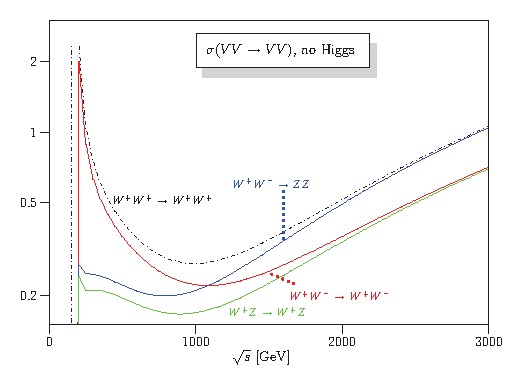
\includegraphics[height=.25\textheight]{figs/ssww_13tev/introduction/vbs_xsec_nohiggs}
  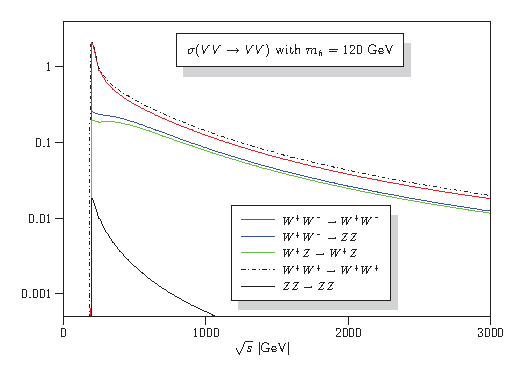
\includegraphics[height=.25\textheight]{figs/ssww_13tev/introduction/vbs_xsec_higgs120}
 
  \caption[Cross sections in nanobarns for five different scattering processes of longitudinally polarized vector bosons as a function of center of mass energy $\sqrt{s}$.  Without a SM Higgs boson (left), the cross sections grow unbounded with $\sqrt{s}$; however with a $120\gev$ Higgs boson (right), the cross sections no longer diverge.]{Cross sections in nanobarns for five different scattering processes of longitudinally polarized vector bosons as a function of center of mass energy $\sqrt{s}$.  Without a SM Higgs boson (left), the cross sections grow unbounded with $\sqrt{s}$; however with a $120\gev$ Higgs boson (right), the cross sections no longer diverge.  Plots taken from~\cite{2008.vbs-resonances-unitarity}.}
  \label{fig:ssww13tev_vbs_xsec_higgs}
\end{figure}

With the discovery of the Higgs boson in 2012~\cite{HIGG-2012-27, CMS-HIG-12-028}, the EWSB mechanism can now be directly studied.
Due to the exchange of a Higgs in the $s$- and $t$-channel VBS diagrams (\ssww itself only contains the $t$-channel diagram), VBS processes are directly sensitive to properties of the Higgs.
For example, the high-mass tail in the $VV$ scattering system allows an approximation of the effective coupling strength of the Higgs to vector bosons that is independent of any assumptions on the Higgs width~\cite{2015.higgs-constraints-from-vbs}.
Additionally, the center of mass energy dependence of the $VV$ scattering can reveal whether the Higgs boson unitarizes the longitudinal scattering amplitude fully or only partially~\cite{2014.higgs-WW-scattering-theory}.

VBS events are characterized by two quarks from the colliding protons each radiating a massive vector boson which then scatter and decay in the detector.
The incoming quarks carry a large amount of momentum and only deflect a small amount upon radiating the vector boson; as a result, they often travel very close to the beam line.
Ignoring the decay products of the bosons, these VBS events result in a final state of two vector bosons ($V$) and two jets ($j$) at high pseudorapidities (called \emph{forward jets}) from the outgoing quarks.
The shorthand $VVjj$ is used to represent this final state.

$VVjj$ events can be produced via two different physical processes.
The first involves purely electroweak interactions in the tree-level diagrams, with $\mathcal{O}(\alpha_{\textrm{EWK}}) = 6$ %(including the decays of the bosons).
and will be referred to as \emph{EWK production}.
This can be further broken down into VBS and non-VBS production.
In the VBS EWK production, the scattering occurs via triple or quartic gauge couplings, as well as the $s$- or $t$-channel exchange of a Higgs boson.
%These diagrams are shown in Figure~\ref{fig:ssww13tev_diagrams_vbs}.
The non-VBS EWK production contains the same final state of two vector bosons and two outgoing quarks, but the bosons do not scatter.
Due to gauge invariance, it is not possible to separate the VBS from the non-VBS productions~\cite{2006.isolating-vbs-lhc}; therefore, both are included in the signal generation and are indistinguishable from one another.
The second process involves a mix of the EWK and strong interactions, of order $\mathcal{O}(\alpha_s) = 2 \otimes \mathcal{O}(\alpha_{\textrm{EWK}}) = 4$ and will be referred to as \emph{QCD production}.
The tree-level Feynman diagrams for VBS EWK, non-VBS EWK, and QCD $VVjj$ production are found in Figures~\ref{fig:ssww13tev_diagrams_vbs}, \ref{fig:ssww13tev_diagrams_ewk}, and \ref{fig:ssww13tev_diagrams_qcd}, respectively.

\begin{figure}[htbp]
  \centering
  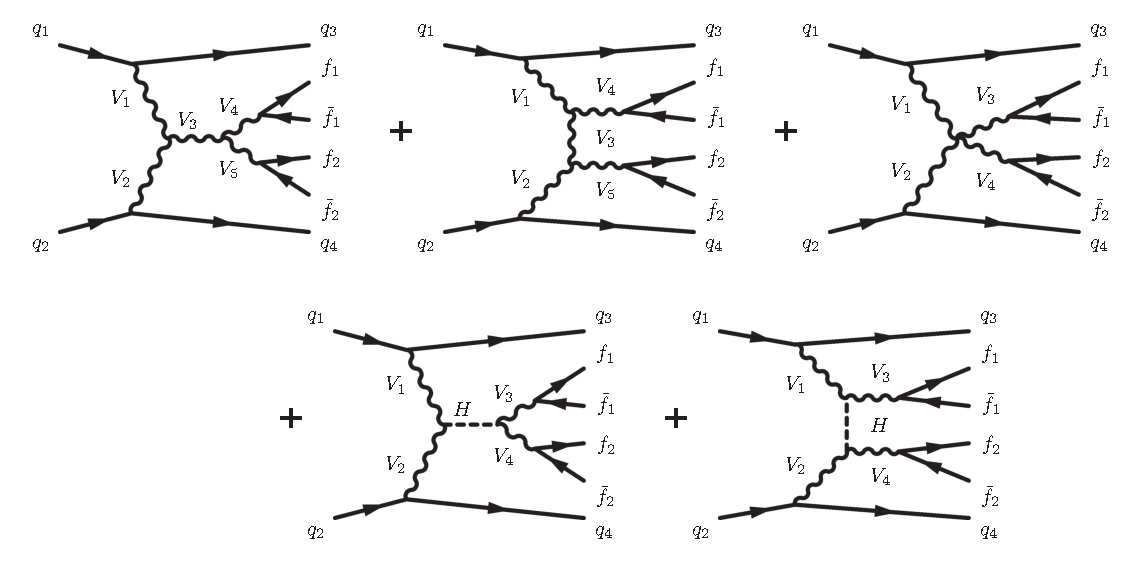
\includegraphics[width=.8\textwidth]{figs/ssww_13tev/diagrams/Vbscore}
  \caption{Tree-level Feynman diagrams for VBS EWK $VVjj$ production including triple gauge couplings involving $W$ and/or $Z$ bosons (top left and top middle), quartic gauge coupling (top right), or the exchange of a Higgs boson ($s$-channel bottom left and $t$-channel bottom right).  The labels are quarks ($q$), fermions ($f$), and gauge bosons ($V = W,Z$).}
  \label{fig:ssww13tev_diagrams_vbs}
\end{figure}

\begin{figure}[htbp]
  \centering
  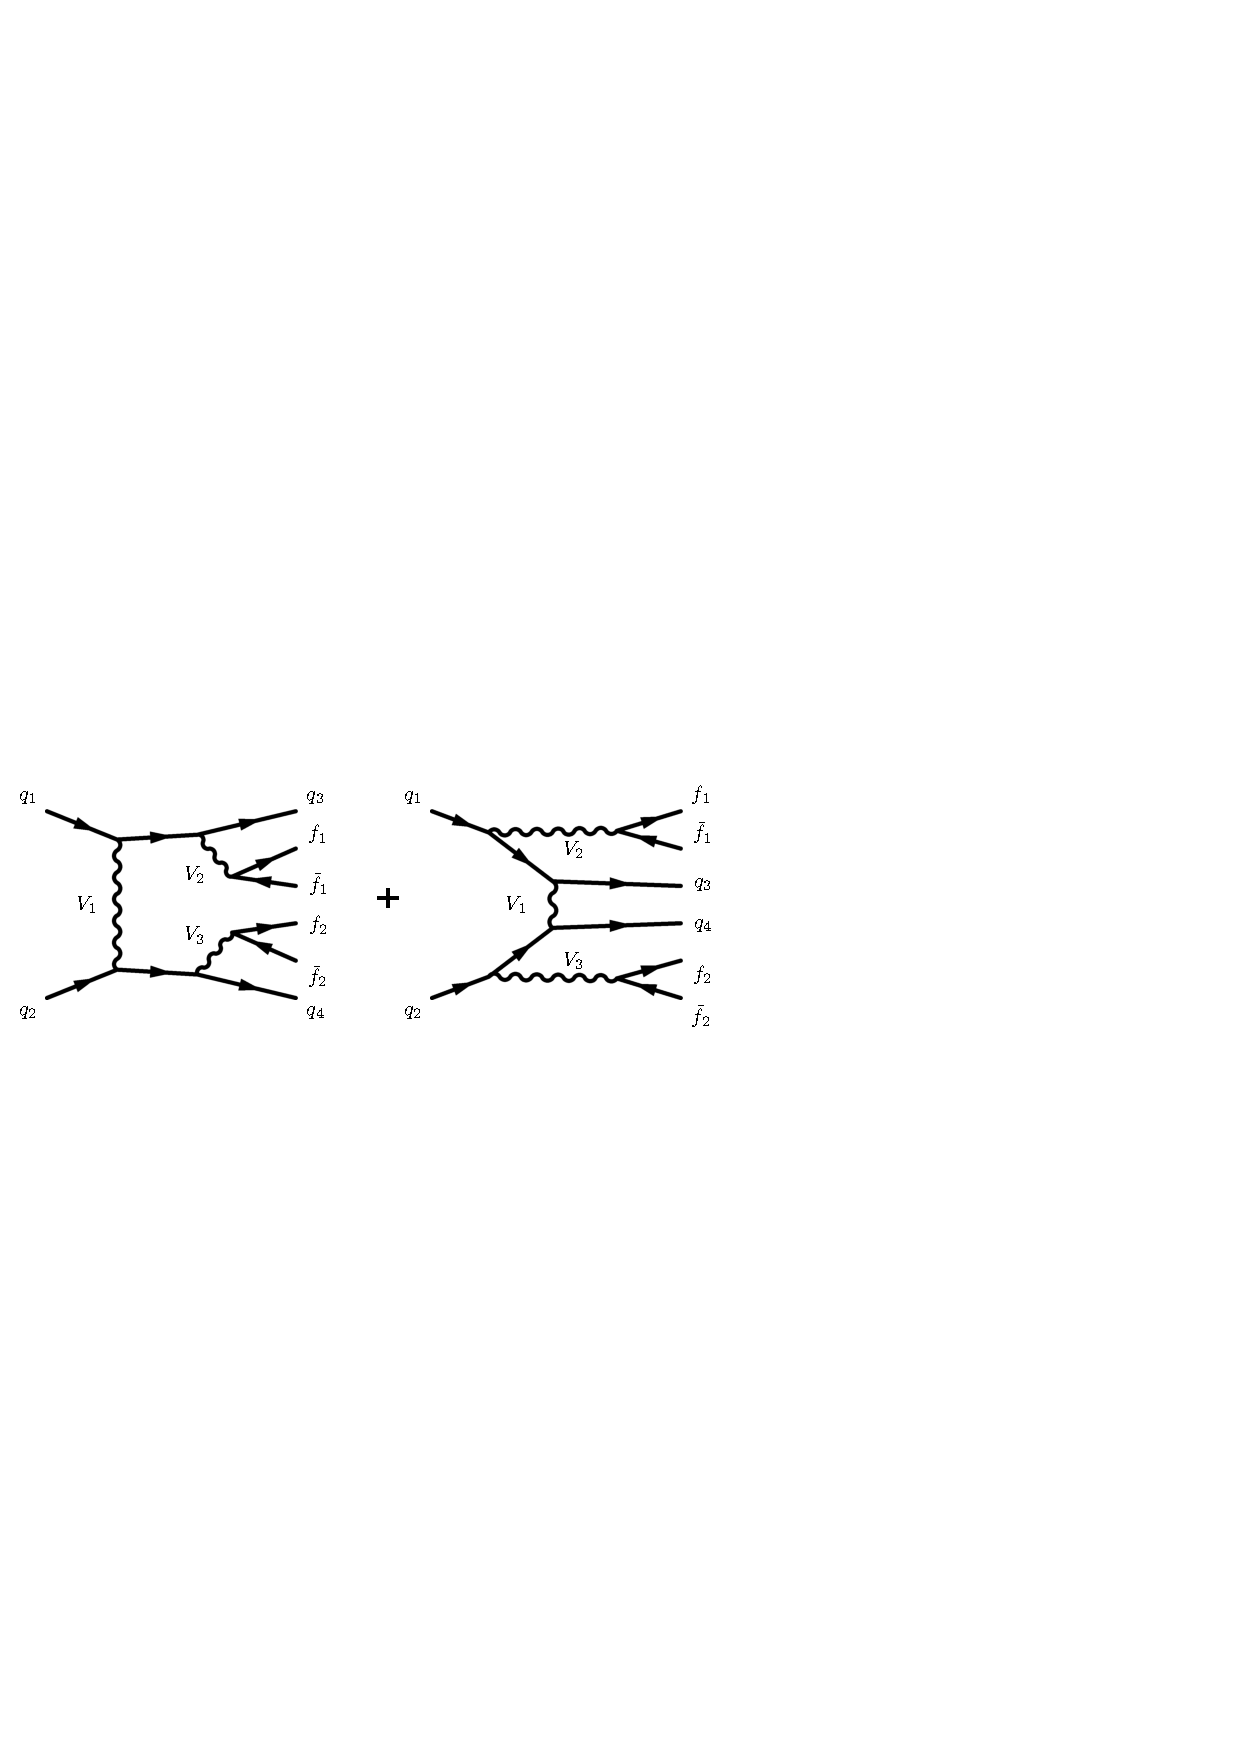
\includegraphics[width=.54\textwidth]{figs/ssww_13tev/diagrams/NoVbsEW}
  \caption{Tree-level Feynman diagrams for non-VBS EWK $VVjj$ production.  The labels are quarks ($q$), fermions ($f$), and gauge bosons ($V = W,Z$).}
  \label{fig:ssww13tev_diagrams_ewk}
\end{figure}

\begin{figure}[htbp]
  \centering
    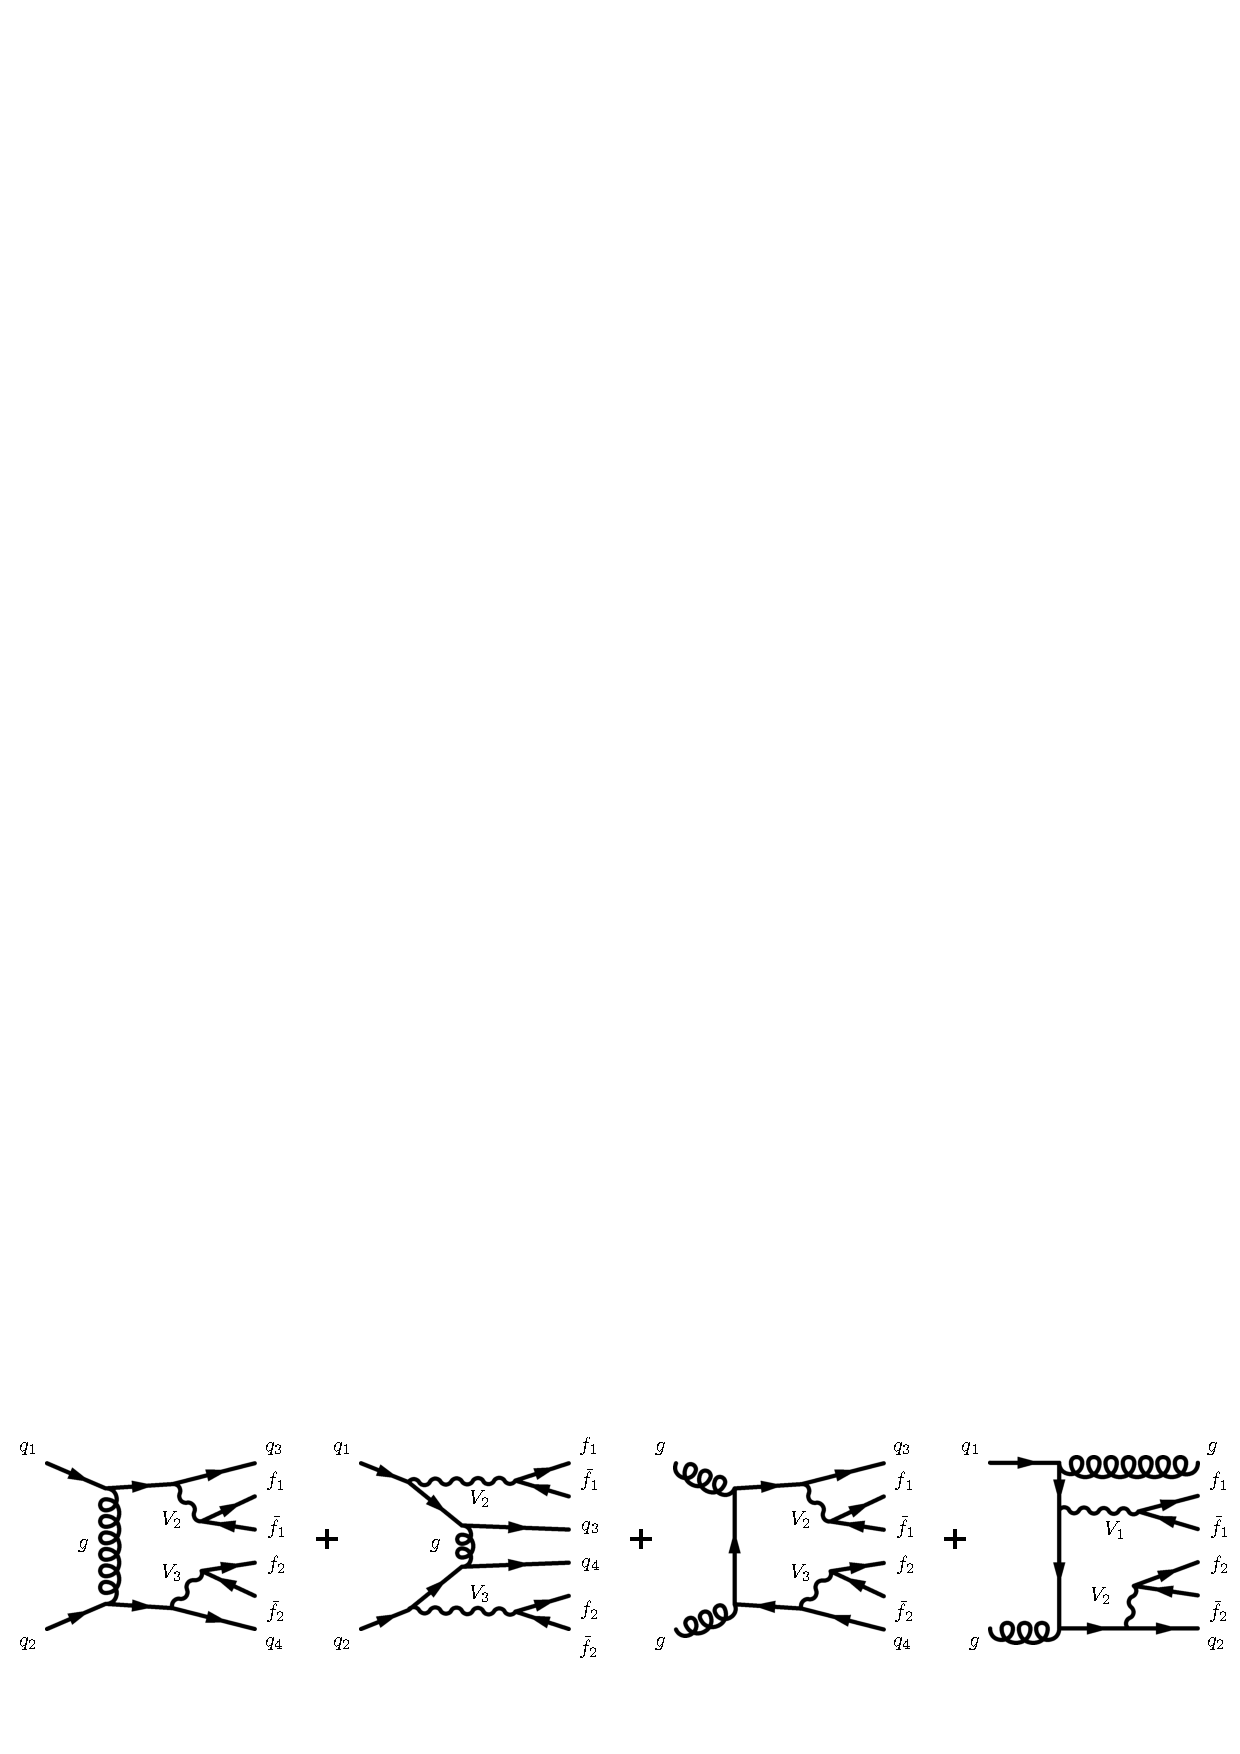
\includegraphics[width=\textwidth]{figs/ssww_13tev/diagrams/VbsQCD}
  \caption{Tree-level Feynman diagrams for QCD $VVjj$ production.  The labels are quarks ($q$), fermions ($f$), and gauge bosons ($V = W,Z$).}
  \label{fig:ssww13tev_diagrams_qcd}
\end{figure}

\subsection{Same-sign $W^{\pm}W^{\pm}$ scattering}\label{ssww13tev:ssww_topology}
Same-sign \ssww scattering is considered to be one of the best channels for studying VBS at the LHC~\cite{2015.higgs-constraints-from-vbs}.
This is due primarily to the ratio of the EWK to the QCD production, which matters a great deal due to the VBS events being a subset of the total EWK production.
In an analysis the EWK production would be conisdered the signal and the QCD production a background, so a favorable ratio of the two helps greatly when comparing the size of the signal to the backgrounds.
A study at \com{8}~\cite{2013.ssww-8tev-atlas-support} was done using the \tt{SHERPA} Monte Carlo (MC) generator to calculate EWK and QCD production cross sections at leading order for a variety of $VVjj$ processes decaying to leptons and can be found in Table~\ref{tab:ssww13tev_qcd_vs_ewk}.
Despite its lower cross section compared to other $VVjj$ processes, the EWK to QCD ratio for \ssww is approximately one-to-one, whereas for opposite-sign \oswwjj the ratio is closer to 3\%.

%There are several advantages to studying the same-sign $WW$ process specifically.
%The final state's net charge of $\pm 2$ helps considerably in reducing the number of background processes that can mimic the signal.

\begin{table}[htbp]
  \centering
  \begin{tabular}{l l r r}
    Process & Final state & $\sigma_{\textrm{EWK}}$ & $\sigma_{\textrm{QCD}}$ \\
    \hline\hline
    $W^{\pm}W^{\pm}$ & $l^{\pm}l^{\pm}\nu\nu jj$    & 19.5 fb & 18.8 fb \\
    $W^{\pm}W^{\mp}$ & $l^{\pm}l^{\mp}\nu\nu jj$    & 91.3 fb & 3030 fb \\
    $W^{\pm}Z$      & $l^{\pm}l^{\pm}l^{\mp}\nu jj$ & 30.2 fb & 687 fb  \\
    $ZZ$          & $l^{+}l^{-}\nu\nu jj$        & 2.4 fb  & 162 fb  \\
    $ZZ$          & $l^{+}l^{-}l^{+}l^{-} jj$     & 1.5 fb  & 106 fb \\
    \hline
  \end{tabular}
  \caption[Predicted cross sections for EQK and QCD production of diboson processes relevant to VBS at \com{8} using the \tt{SHERPA} MC generator.  Loose generator level cuts are applied on lepton $\pt > 5\gev$, dilepton invariant mass $m_{ll} > 4\gev$, and at least two jets with $m_{jj} > 10\gev$.]{Predicted cross sections for EQK and QCD production of diboson processes relevant to VBS at \com{8} using the \tt{SHERPA} MC generator.  Loose generator level cuts are applied on lepton $\pt > 5\gev$, dilepton invariant mass $m_{ll} > 4\gev$, and at least two jets with $m_{jj} > 10\gev$.  Numbers taken from~\cite{2013.ssww-8tev-atlas-support}.}
  \label{tab:ssww13tev_qcd_vs_ewk}
\end{table}

This analysis studies \ssww scattering where both $W$ bosons decay leptonically to $e\nu$ or $\mu\nu$\footnote{Throughout the rest of this chapter, $l$ denotes either electrons ($e$) or muons ($\mu$) unless stated otherwise.  Additionally, $e$, $\mu$, and $\nu$ (neutrino) with no charge or anti-particle designation refer interchangeably to either the particle or anti-particle.}.
The \ssww VBS final state consists of two leptons with the same electric charge, two neutrinos, and two high energy forward jets with a large invariant mass.
Tree-level Feynman diagrams of VBS \ssww production can be found in Figure~\ref{fig:ssww13tev_diagrams_vbs_ssww} and a visual representation of the VBS topology can be found in Figure~\ref{fig:ssww13tev_event_topology}.
The two forward jets also serve as a powerful tool to suppress the QCD production mode.
In EWK events, the two jets tend to have much higher separation and a larger combined invariant mass than the two leading jets in a QCD event.
The two plots shown in Figure~\ref{fig:ssww13tev_dijet_comparison} highlight the differences in these dijet quantities between the two production modes.
An ATLAS event display of a real \ssww candidate event is shown in Figure~\ref{fig:ssww13tev_event_display_mm}.

% i think i really only need to include the vbs diagrams for ssww (maybe also the ewk?) since the general VV ones are above for all processes
\begin{figure}[htbp]
  \centering
  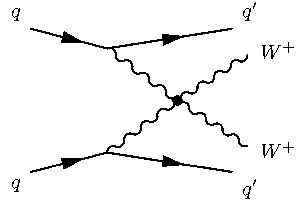
\includegraphics[width=.32\textwidth]{figs/ssww_13tev/diagrams/vbs1}
  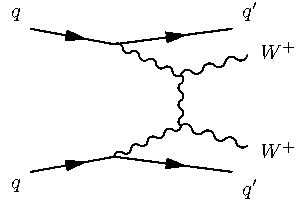
\includegraphics[width=.32\textwidth]{figs/ssww_13tev/diagrams/vbs2}
  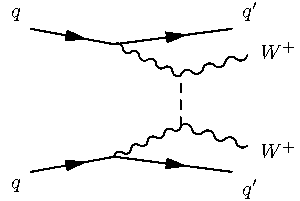
\includegraphics[width=.32\textwidth]{figs/ssww_13tev/diagrams/vbs3}
  \caption{Feynman diagrams for VBS EWK production of \ssww events. The leftmost diagram contains a quartic gauge coupling vertex, and the rightmost diagram contains an exchange of a Higgs boson. \TODO{Make diagrams consistent with others}}
  \label{fig:ssww13tev_diagrams_vbs_ssww}
\end{figure}

\begin{figure}[htbp]
  \centering
  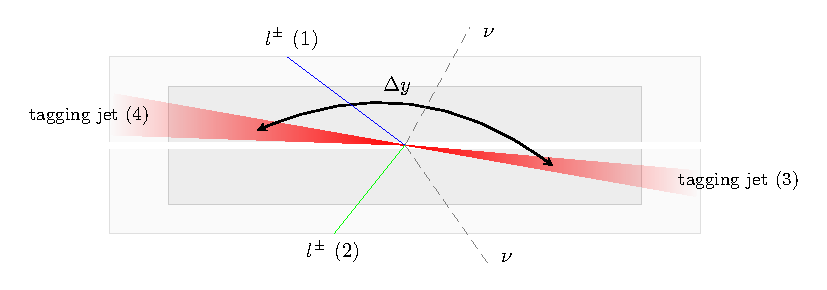
\includegraphics[width=.95\textwidth]{figs/ssww_13tev/introduction/vbs_event_topology}
  \caption{\ssww VBS event topology containing two leptons (1 and 2) with the same electric charge, two neutrinos, and two forward tagging jets (3 and 4) with large rapidity separation $\Delta y$.}
  \label{fig:ssww13tev_event_topology}
\end{figure}

\begin{figure}[htbp]
  \centering
  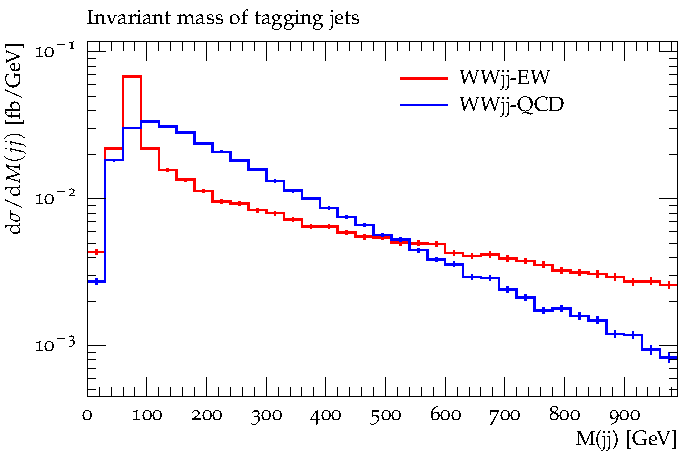
\includegraphics[width=.48\textwidth]{figs/ssww_13tev/introduction/Nm1_mjj}
  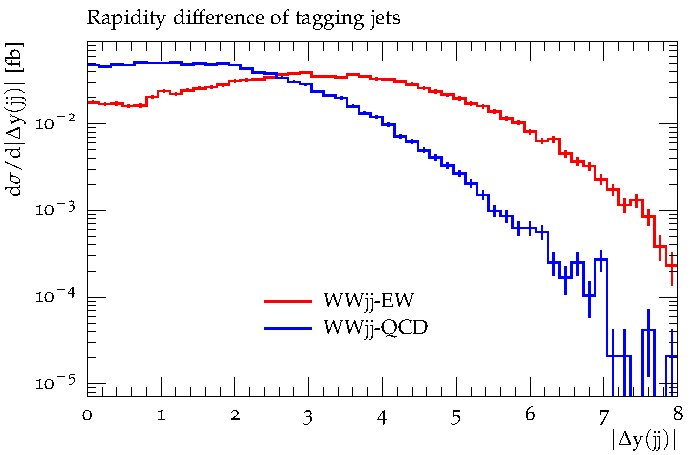
\includegraphics[width=.48\textwidth]{figs/ssww_13tev/introduction/Nm1_deltaY}
  \caption[Generator level comparisons at \com{8} of dijet invariant mass ($m_{jj}$, left) and dijet rapidity ($\Delta y_{jj}$, right) in EWK (red) and QCD (blue) \ssww events.  Both data sets have been normalized to the same area.]{Generator level comparisons at \com{8} of dijet invariant mass ($m_{jj}$, left) and dijet rapidity ($\Delta y_{jj}$, right) in EWK (red) and QCD (blue) \ssww events.  Both data sets have been normalized to the same area.  Plots taken from~\cite{2013.ssww-8tev-atlas-support}.}
  \label{fig:ssww13tev_dijet_comparison}
\end{figure}

\begin{figure}[htbp]
  \centering
  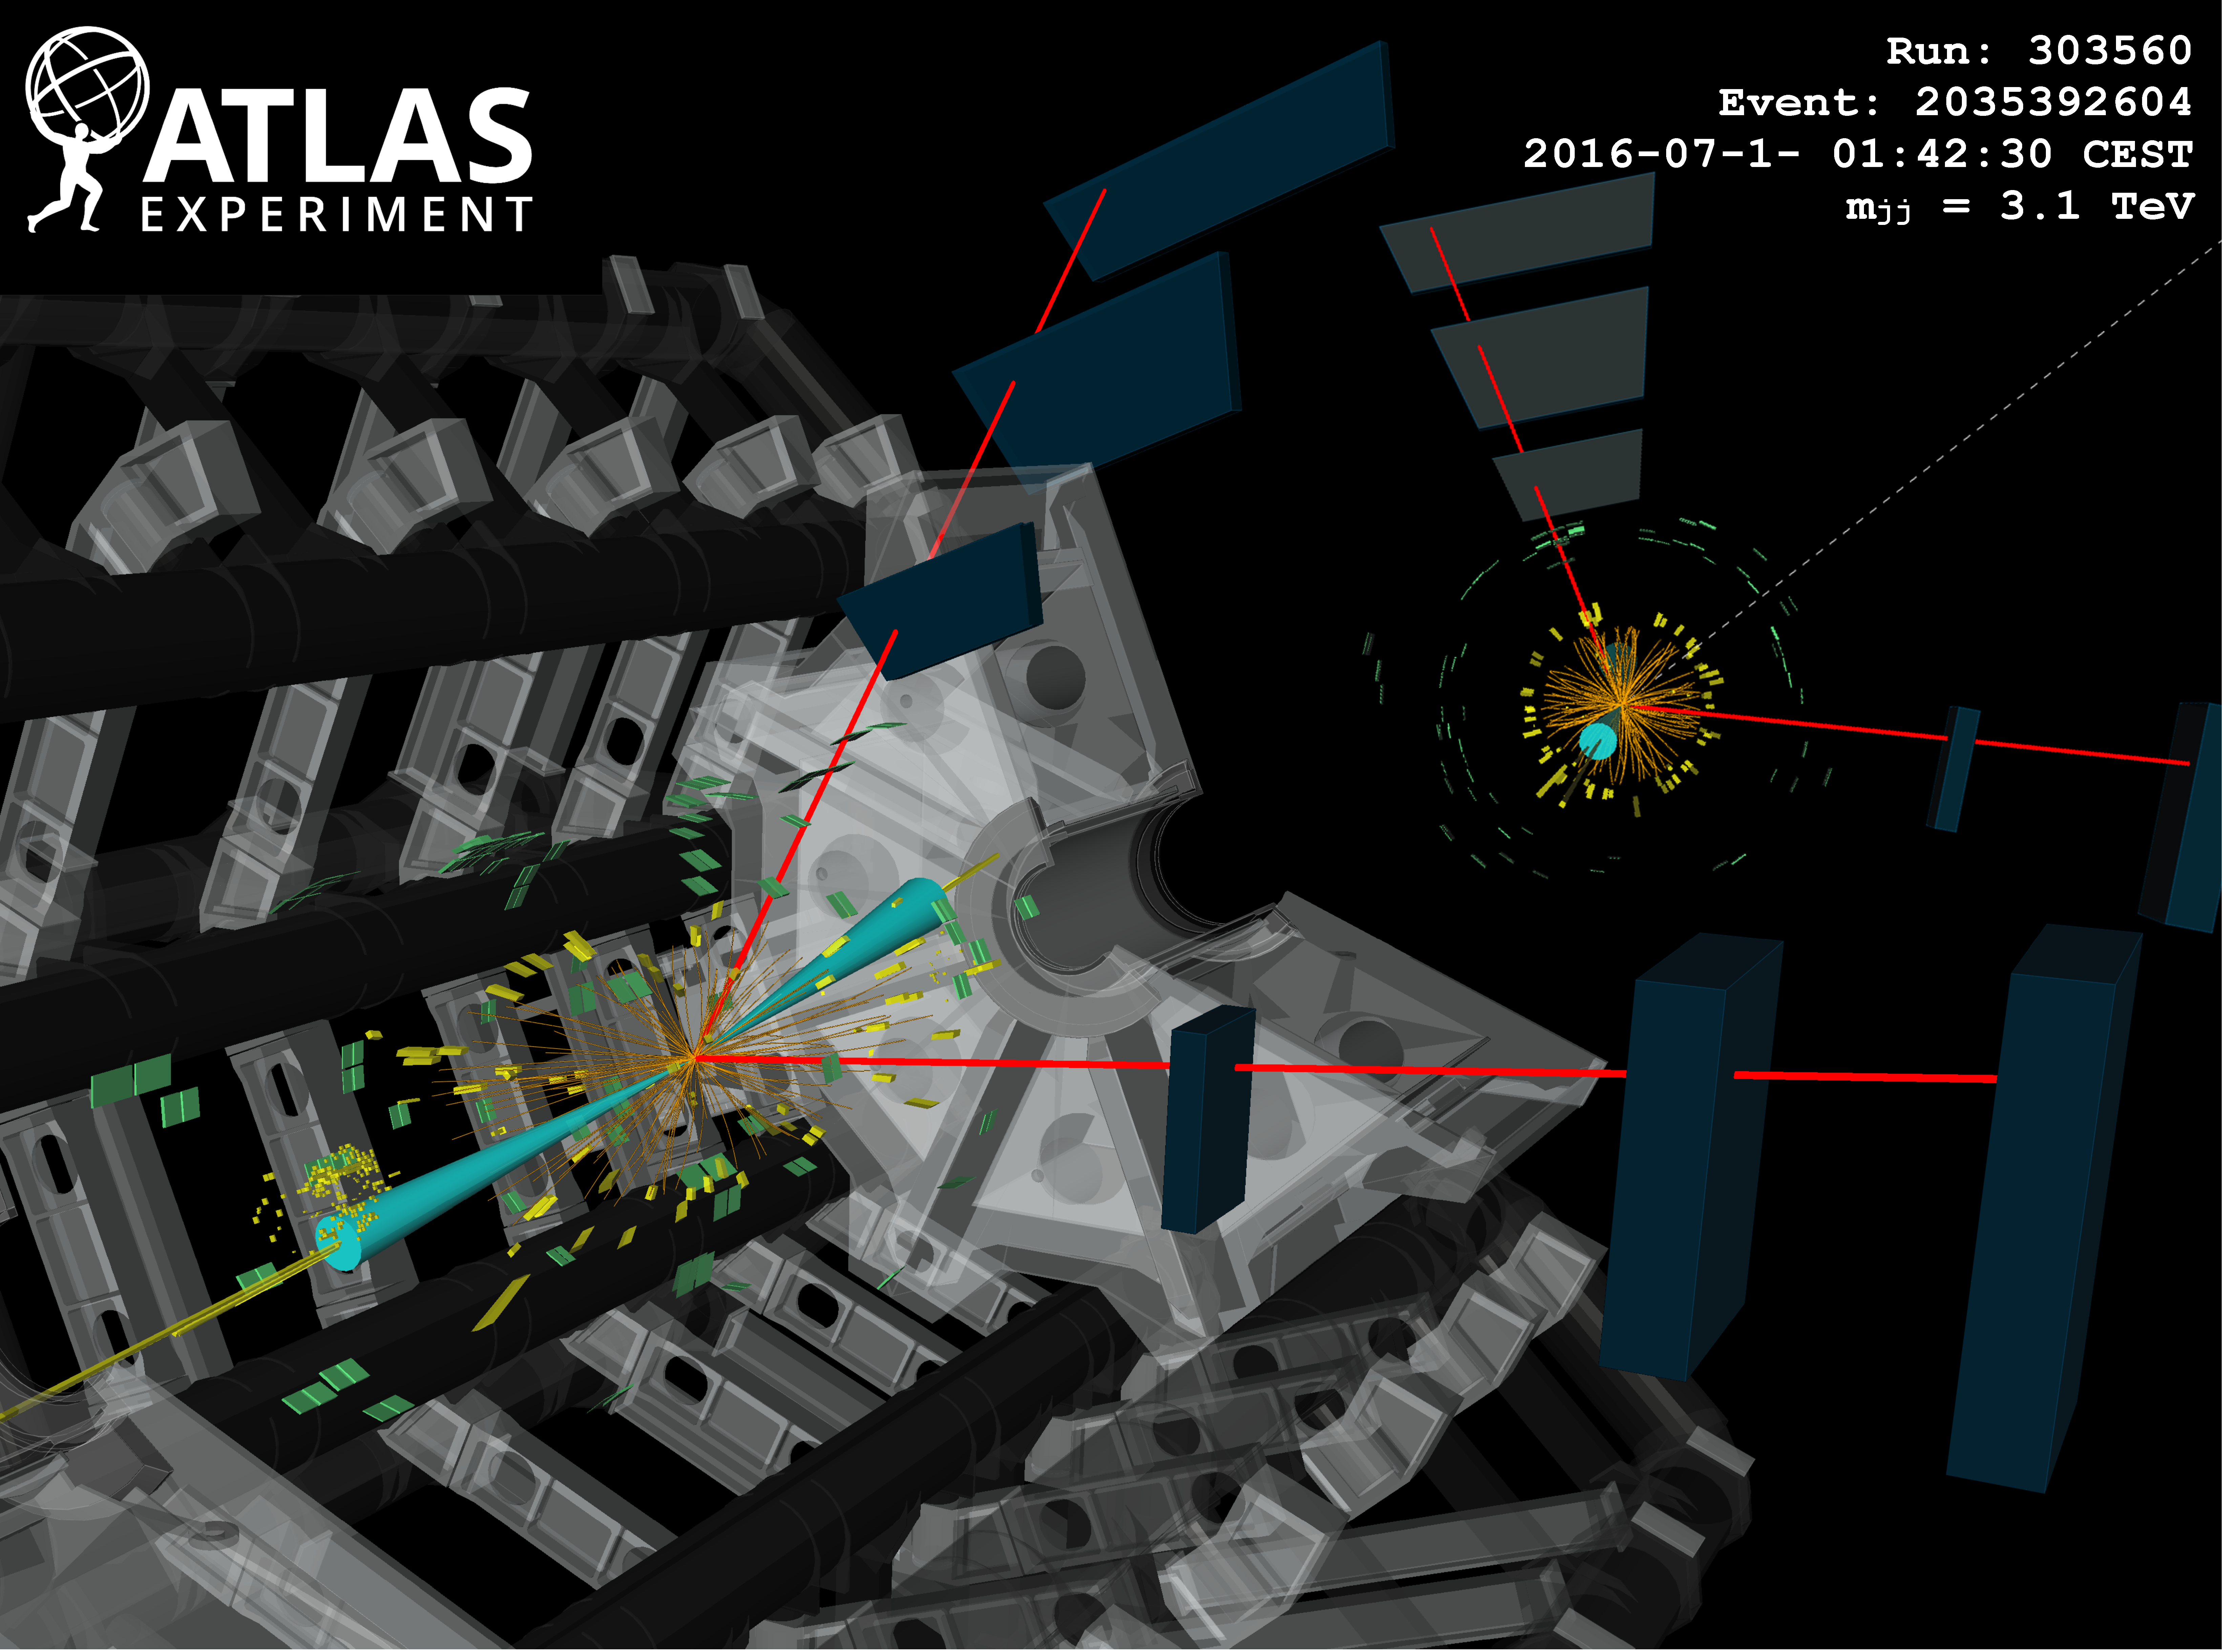
\includegraphics[width=.95\textwidth]{figs/ssww_13tev/introduction/evtdisplay_mm}
  \caption{ATLAS event display of a $pp\rightarrow W^{+}W^{+}\rightarrow\mu^{+}\nu_\mu\mu^{+}\nu_\mu jj$ event.  The muons are represented by the red lines travelling from the ID through the MS, and the forward jets are represented by the blue cones with yellow energy deposits in the calorimeters.  The direction of the $\met$ in the transverse plane is indicated by the gray dashed line in the inset image.  Event display taken from~\cite{2018.ssww-13tev-atlas-conf}.}
  \label{fig:ssww13tev_event_display_mm}
\end{figure}

\subsection{Overview of backgrounds}\label{ssww13tev:background_overview}
In addition to QCD production of \ssww events, there are several other processes that can end up with a final state of two same-sign leptons, two neutrinos, and two jets.
However, due to the $\pm 2$ final state charge, there is a considerable reduction in SM backgrounds (such as $Z$ boson events) when compared to an analysis like opposite-sign \oswwjj.

One of the largest sources of background involves processes with prompt leptons\footnote{Prompt leptons are those that are produced in the primary collision and are a direct decay product of the process of interest.  Non-prompt leptons originate from some secondary process, such as a $b$-hadron decay, or are jets that get mis-reconstructed as a lepton.}.
These are events that contain two leptons with the same electric charge and one or more additional leptons that are ``lost'', either by failing the selection criteria or falling outside of the detector's acceptance.
The number of processes that can contribute is limited by the requirement of same-sign leptons, and as a result this background is dominated by processes involving two or more vector bosons, with the largest contribution coming from $WZ$ events and smaller contributions from $ZZ$ and $t\bar{t}V$ events.
Triboson events where one boson decays hadronically also contribute to this background; however, the jets are generally softer and more central than in a typical VBS event, and the cuts applied on the forward jets suppress these contributions.

The other dominant background comes from non-prompt, or ``fake'', leptons.
Here one or more leptons originate from the decay of another particle unrelated to the signal process, such as a heavy-flavor decay or photon conversion, or come from a jet that is misidentified as a lepton.
This background is mostly made up of events from $t\bar{t}$ and $W$+jets processes, with a much smaller contribution from $V\gamma$ events. \TODO{check whether $V\gamma$ really qualifies as non-prompt, we lump $Z\gamma$ in with the charge flip background in the paper...}

Finally, opposite-sign lepton pairs can enter the signal region if one of the leptons is reconstructed with the wrong charge (called \emph{charge misidentification}\footnote{Charge misidentification is also referred to interchangeably as \emph{charge mis-ID} and \emph{charge flip}.}).
In practice, this only affects events with electrons, as the charge misidentification rate for muons is negligible~\cite{2013.muon-flip}.
This is a major background in events with two electrons, but is a much smaller contribution for events with one electron and one muon.

%\subsection{}\label{ssww13tev:theory}
%Hello world!

